\documentclass[11pt, a4paper]{article}
%\usepackage[round]{natbib}

\usepackage{mathtools}
\usepackage{setspace} 
\usepackage{dsfont}
\usepackage{amsfonts}
\usepackage{amsmath}
\usepackage{subcaption}
\usepackage{paralist}
%\usepackage{subfig}
\usepackage{times}  
\usepackage{latexsym}
\usepackage{graphicx}
\usepackage[T1]{fontenc}
\usepackage{tikz}
\usepackage{url}
\usepackage{pgfplotstable}
\usepackage{titlesec}
\usepackage{color}
\usepackage{lipsum,adjustbox}
\usepackage{bbm}
\usepackage{booktabs}


\usepackage{xr}
\externaldocument[]{conservatism_supplementary}
\makeatletter
\newcommand{\@BIBLABEL}{\@emptybiblabel}
\newcommand{\@emptybiblabel}[1]{}
%\makeatother
\usepackage[hidelinks]{hyperref}
%\setlength{\parskip}{-.em}

\usepackage{acl2018}
\graphicspath{{./plots/}}
\newcommand{\com}[1]{}
%\newcommand{\oa\part{title}}[1]{}
%\newcommand{\lc}[1]{}
%\newcommand{\oa}[1]{}
\newcommand{\oa}[1]{\footnote{\color{red}OA: #1}}
\newcommand{\oamod}[1]{{\color{red}#1}}
\newcommand{\lc}[1]{\footnote{\color{blue}LC: #1}}
\newcommand{\lcmod}[1]{{\color{blue}#1}}

\newenvironment{myequation}{
  \vspace{-1em}
 \begin{equation}
}{
 \end{equation}
 \vspace{-1.2em}
}
\newenvironment{myequation*}{
	\vspace{-1em}
	\begin{equation*}
}{
\end{equation*}
\vspace{-1.2em}
}
\aclfinalcopy 

\begin{document}
\title{Inherent Biases in Reference-based Evaluation for \\ Grammatical Error Correction and Text Simplification}
\author{
  Leshem Choshen\textsuperscript{1} and Omri Abend\textsuperscript{2} \\
  \textsuperscript{1}School of Computer Science and Engineering,
  \textsuperscript{2} Department of Cognitive Sciences \\
  The Hebrew University of Jerusalem \\
  \texttt{leshem.choshen@mail.huji.ac.il, oabend@cs.huji.ac.il}\\
}
\maketitle

	\begin{abstract}
		The prevalent use of too few references for evaluating text-to-text
		generation is known to bias estimates of their quality (henceforth, {\it low
		  coverage bias} or LCB). This paper shows that overcoming LCB in
		Grammatical Error Correction (GEC) evaluation cannot be attained by
		re-scaling or by increasing the number of references in any feasible
		range, contrary to previous suggestions. This is due to the long-tailed distribution of valid corrections for a sentence.
		Concretely, we show that LCB incentivizes GEC systems to avoid
    correcting even when they can generate a valid correction. 
    Consequently, existing systems obtain comparable or
		superior performance compared to humans, by making few but targeted 
		changes to the input.
		Similar effects on Text Simplification further support our claims.
	\end{abstract}

	%\vspace{-.2cm}
	\section{Introduction}
	%\vspace{-.2cm}
	
	\lc{originally we wanted to move some TS text from the supplementary to here, given the reviews (stating we are too dense) should we reconsider? Do we have a way of a last effort for making the article easier to comprehend, I will make another iteration but am skeptical?}
	Evaluation in monolingual translation \cite{xu2015problems,inderjeet2009summarization} and
	in particular in GEC
	\cite{tetreault2008native,madnani2011they,felice2015towards,bryant2015far,napoles2015ground}
	has received much attention over the years, and has gained notoriety for its difficulty,
	due in part to the heterogeneity of the space of valid corrections \cite{chodorow2012problems}, this it also the case in machine translation (MT) \cite{dreyer2012hyter}.
	Most common evaluation measures for GEC are reference-based measures (RBM), including
  $M^2$ \cite{dahlmeier2012better}, which is the de-facto standard, GLEU \cite{napoles2015ground} and I-measure \cite{felice2015towards}.
	
  The Inadequate Coverage Bias (LCB) was previously discussed by \citet{bryant2015far}, 
  who showed that inter-annotator agreement in producing references is low, 
  and concluded that RBMs under-estimate the performance of GEC systems.
  To address this, they proposed a new measure, Ratio Scoring, which re-scales $M^2$ 
  by the inter-annotator agreement (i.e., the score of a human corrector), interpreted as an upper bound.

  In this paper, we revisit the LCB, and show it has more far-reaching implications than previously discussed. 
  First, while we agree with \citet{bryant2015far} that a human correction should receive a perfect score, 
  we show that LCB does not merely scale system performance by a constant factor, but
  rather that some correction policies are less prone to be biased against. 
  Concretely, we show that by only correcting closed class errors, where few possible corrections are valid, systems can outperform humans. 
  Indeed, in Section \ref{sec:real_world} we show that some existing systems outperform humans on $M^2$ and GLEU, while only applying few changes to the source.
  
  We thus argue that the development of GEC systems against low coverage RBMs disincentivizes systems from making changes to the source 
  in cases where there are plentiful valid corrections (open class errors), as necessarily only some of them are covered by the reference set. 
  To support our claim we show that (1) existing GEC systems under-correct, often performing an order of magnitude less corrections than a human does (\S\ref{subsec:under-correction});
  (2) increasing the number of references alleviates under-correction (\S\ref{subsec:reranking});
  and (3) under-correction is more expressed in error types that are more varied in their valid corrections (\S\ref{subsec:by_types}).
  
  Recent work has also attempted to address LCB by increasing the number of references 
  (henceforth, $M$) \cite{bryant2015far,sakaguchi2016reassessing}.
  In Section \ref{sec:increase-reference} we estimate the distribution of corrections per sentence, 
  and find that increasing $M$ is unlikely to overcome LCB, due
  to the vast number of valid corrections for a sentence and their long-tailed distribution.
  Indeed, even short sentences have over 1000 valid corrections on average. 
  We also assess the effect of increasing $M$ on 
  the score of a perfect system (i.e., the inter-annotator agreement) 
  using $M^2$, accuracy and GLEU, finding diminishing returns. 

  In order to corroborate our findings, we apply a 
  similar line of experiments to Text Simplification (TS) (\S\ref{sec:simplification}),
  finding similar trends: (1) the distribution of valid simplifications for a given sentence is long-tailed; 
  (2) common measures for TS dramatically under-estimate performance; 
  (3) additional references alleviate this under-prediction.
  %\lc{I think we should rephrase, lets call over-conservatism only the strictly 
  %wrong conservatism (e.g. choosing a wrong sentence  
  %from k best list) and refer to very conservative systems that are presumably over conservative}.
  %Indeed, over-conservatism has been reported by a number of recent works on TS.

  To recap, we find that the LCB hinders the reliability of RBMs for GEC,
  and incentivizes systems developed to optimize these measures not to correct. 
	LCB cannot be overcome by re-scaling or increasing $M$ in any feasible range. 
  %We conclude by discussing issues with existing metric validation methodology, and outlining 
  %paths for future advancement (\S\ref{sec:conclusion}).
  

  
  
  %While we present 
  %  (\S \ref{sec:real_world}) the methodology to report confidence bounds for correctors' performance we show some of them already surpass human performance in the task.
	
  %	In section \ref{sec:formal_conservatism} we discuss why, given the aforementioned high system performance, LCB is not solved by RS. We show analytical and empirical results supporting the claim that LCB  results in correctors avoiding corrections even when they have high probability of correcting well, or have a valid correction in a $k$-best list. This is because RBMs in general and more severely precision oriented ones penalize valid corrections. Furthermore, we are the first to show that 15 current correctors including the supposedly better than human ones hardly correct at all, which we presume is at least partially due to the biases.
	

%An important criterion in GEC evaluation is faithfulness to the source. 
%In fact, some argue that a somewhat cumbersome or even mildly ungrammatical 
%correction if preferable over one that alters the meaning of the source \cite{brockett2006correcting}.
%Consequently, annotators are often instructed to be conservative when compiling gold standard corrections \cite[e.g.,][]{nicholls2003cambridge}.
%Several evaluation procedures have attempted to formally capture this precision/recall asymmetry,
%such as the standardized use of $F_{0.5}$ over $F_{1}$ \cite{ng2014conll} and the 
%choices of weights in I-measure \cite{felice2015towards}.

%However, penalizing over-correction more harshly than under-correction during development and training, 
%may lead to reluctance of correctors to make any changes (henceforth, {\it over-conservatism}).
%Using only one or two reference corrections, the common practice in GEC, compounds this problem,
% as correctors are not only harshly penalized for making incorrect changes, but are often penalized
%for making correct changes not found in the reference.

%Indeed, we show that state-of-the-art correctors present over-conservatism.
%Evaluating the output of 15 recent correctors, we find they all
%substantially under-predict corrections relative to the already conservative references
%(\S\ref{sec:formal_conservatism}).
%Differences in the prevalence of changes in the outputs and in the references are often an order of magnitude large, and are unlikely to be desirable (\S\ref{sec:increase-reference}).

%We first assess the effect of increasing the number of references (henceforth, $M$) on 
%the undue penalization of valid corrections (\S \ref{sec:increase-reference}).
%We start by estimating the number and frequency distribution of the valid corrections per sentence, arriving 
%at an estimate of over 1000 corrections, even for fairly short sentences.
%We then consider two representative reference-based measures (henceforth, {\it RBMs}) to
%assess the validity of a proposed correction relative to a reference set, 
%and characterize the distribution of their scores as a function of $M$. 
%Our results show that both measures substantially under-estimate the true performance of
%the correctors. They also show that increasing $M$ alleviates the incurred bias, 
%and reduces over-conservatism. All this suggests developing, tuning and training correctors against a larger number of valid corrections is likely to reduce over-conservatism.
%However, as increasing $M$ shows diminishing returns, a compelling alternative
%is to leverage recent advances in semantic parsing to define semantic
%measures to supplement RBMs (\S\ref{sec:conclusion}). 


%Specifically, we introduce in another paper sent to this conference GEC RLM to assess the extent to which
%a correction faithfully represents the semantics of the source, by their semantic structures similarity(\S \ref{sec:Semantics}).
%This approach can be combined with RLM based on grammatical error detection(GED), as proposed by \newcite{napoles-sakaguchi-tetreault:2016:EMNLP2016}.
%
%Our experiments support the feasibility of the proposed approach,by showing that (1) semantic structural annotation can be consistently and automatically applied to LL, (2) that the proposed measure is less prone to unduly penalize valid corrections and (3) that the measure does penalize corrections that alter the semantic structure significantly.
%
%
%
%We define a measure, using the UCCA scheme \cite{abend2013universal} as a
%test case, motivated by its recent use for machine translation
%evaluation \cite{birch2016hume}.
%We annotate a section of the NUCLE parallel corpus \cite{dahlmeier2013building},
%
%The two approaches address the insufficiency of using too few references from
%complementary angles. The first attempts to cover more of the probability
%mass of valid corrections by taking a larger $M$, 
%while the second uses semantic instead of string similarity, in order
%to abstract away from some of the formal variation between different valid corrections.
%
%

%%%%%%%%%%%%%%%%%%%%%%%%%%%%%%%%%%%%%%%%%%%%%%%%%%%%%%%%%%%%%%%%%%%%%%%%%%%%%%
%\vspace{-.2cm}
\section{Coverage in RBMs}\label{sec:increase-reference}
%\vspace{-.1cm}

We begin by formulating a methodology for studying the distribution of valid 
corrections for a sentence (\S\ref{subsec:corrections_distribution}), 
and then turn to assessing the effect inadequate 
coverage has on common RBMs (\S\ref{subsec:Assessment-values}). 
Finally, we compare human and system scores by common RBMs (\S\ref{sec:real_world}).

%We then proceed to discuss the relation between  references and the behaviour of RBMs.
%To open the discussion we put forward an analysis of some of GEC fundamental properties. 
%We create a methodology and estimate the distribution of valid corrections allowing for better understanding of the task we face when trying to correct corrections. 

%\vspace{-.1cm}
\paragraph{Notation.}
We assume each ungrammatical sentence $x$ has a set of valid corrections $Correct_x$,
and a discrete distribution $\mathcal{D}_x$ over them, where $P_{\mathcal{D}_x}(y)$
for $y \in Correct_x$ is the probability a human annotator would correct $x$ as $y$.

Let $X=x_{1}\ldots x_{N}$ be the evaluated set of source sentences and denote $\mathcal{D}_{i}\coloneqq \mathcal{D}_{x_i}$. Each $x_{i}$ is independently sampled from some 
distribution $\mathcal{L}$ over input sentences, 
and is paired with $M$ corrections $Y_i = \left\{y_{i}^{1},\ldots, y_{i}^{M}\right\}$,
which are independently sampled from $\mathcal{D}_{i}$. Our analysis assumes a fixed number of references across sentences, 
but generalizing to sentence-dependent $M$ is straightforward.
The {\it coverage} of a reference set $Y_i$ of size $M$ for a sentence $x_i$ is defined as $P_{y \sim \mathcal{D}_i}(y \in Y_i)$.

A system $C$ is a function from input sentences to proposed corrections (strings).
An evaluation measure is a function $f\colon X \times Y \times C\to \mathbb{R}$. We use the term 
``true measure'' to refer to a measure's output where the reference set includes all valid corrections, 
i.e., $\forall i\colon Y_i=Correct_i$.

%\vspace{-.2cm}
\paragraph{Experimental Setup.}\label{par:experimental_setup}
We conduct all experiments on the NUCLE test dataset \cite{dahlmeier2013building}.
NUCLE is a parallel corpus of essays written by language learners and their corrected versions,
containing 1414 essays and 50 test essays, each of about 500 words.

We evaluate all participating systems in the CoNLL 2014 shared task,
in addition to three of the best performing systems on this dataset,
a hybrid system \cite{rozovskaya2016grammatical},
a phrase-based MT system \cite{junczysdowmunt-grundkiewicz:2016:EMNLP2016} 
and a neural network system \cite{xie2016neural}.
Appendix  \ref{ap:abbr} lists system names and abbreviations.

%
	%\vspace{-0.1cm}
\subsection{Estimating the Corrections Distribution}\label{subsec:corrections_distribution}
	%\vspace{-0.1cm}
%
\paragraph{Data.}
We turn to estimating the number of corrections per sentence, and their histogram.
The experiments in the following section are run on a random sample of 52 short sentences from the NUCLE test data, i.e. with 15 words or less. Through the length restriction, we avoid introducing too many independent errors that may drastically increase the number of annotation variants (as every combination of corrections for these errors is possible), thus resulting in unreliable estimation for $\mathcal{D}_x$. 

Proven effective in GEC and related tasks such as MT \cite{zaidan2011crowdsourcing,madnani2011they,post2012constructing}, 
we use crowdsourcing to sample from $\mathcal{D}_x$ (see Appendix  \ref{ap:crowd}).
Aiming to judge grammaticality rather than fluency, we instructed the workers to correct only when necessary, not for styling.
We begin by estimating the histogram of $\mathcal{D}_x$ for each sentence, using the crowdsourced corrections.
We use {\sc UnseenEst} \cite{zou2015quantifying}, a non-parametric algorithm to
estimate a discrete distribution in which the individual values do not matter, only their probability. 
{\sc UnseenEst} aims to minimize the ``earthmover distance'', between the estimated histogram and the histogram of the distribution. 
Intuitively, if histograms are piles of dirt, {\sc UnseenEst} minimizes the amount of dirt moved times the distance it moved.
{\sc UnseenEst} was originally developed and tested for estimating the histogram of
variants a gene may have, including undiscovered ones, a setting similar to ours.
%This is a similar setting to the one tackled here.
\lc{Organize git}
Our manual tests of {\sc UnseenEst} with small artificially created datasets
showed satisfactory results.\footnote{An implementation of \href{https://github.com/borgr/unseenest}{\sc UnseenEst}, the data we collected, the estimated distributions and efficient implementations of ways to deal with \href{https://github.com/borgr/PoissonBinomial}{poisson binomial distributions} can be found in \url{https://github.com/borgr/IBGEC}.}

Our estimates show that most input sentences have a large number of
infrequent corrections that account for much of the probability mass
and a rather small number of frequent corrections.
%The estimated distributions tend to have steps, with many corrections with the same (low) frequency.
Table \ref{tab:corrections_dist} presents the mean number of different corrections with frequency at least $\gamma$ (for different $\gamma$s), and their total probability mass.
For instance, 74.34 corrections account for 75\% of the probability mass, each occurring with frequency $\geq$ 0.1\%.

\begin{table}[h!]
	%\vspace{-0.5cm}
  \centering
  \small
  \singlespacing
  \begin{tabular}{c|c|c|c|c|}
    %\cline{2-5} 
    & \multicolumn{4}{c|}{Frequency Threshold ($\gamma$)}\\ 
    %\cline{2-5} 
    & \multicolumn{1}{c}{0} & \multicolumn{1}{c}{0.001} & \multicolumn{1}{c}{0.01} & \multicolumn{1}{c|}{0.1}
    \\
    \hline
    Variants & 1351.24 & 74.34 & 8.72 & 1.35
    \\
    Mass & 1 & 0.75 & 0.58 & 0.37\\
    \hline
  \end{tabular}
  \caption{\label{tab:corrections_dist}
    Estimating the distribution of corrections $\mathcal{D}_x$.
    The table presents the mean number of corrections per sentence with probability more than
    $\gamma$ (top row), as well as their total probability mass (bottom row).
  }
  %\vspace{-0.3cm}
\end{table}

The high number of rare corrections raises the question of whether these can be regarded as noise.
To test this we conducted another crowdsourcing experiment, where 3 annotators were asked to judge whether a correction produced in the first experiment, is indeed valid.
%Figure \ref{fig:validity_judgements} presents the frequency in which annotators judged a correction to be valid, where corrections are binned by the number of workers who generated them.
We plot the validity of corrections against their frequencies, finding that frequency has little effect,
where even the rarest corrections are judged valid 78\% of the time.
Details in Appendix \ref{ap:validity_judgements}.

%\vspace{-.2cm}
\subsection{Under-estimation as a Function of $M$} \label{subsec:Assessment-values}
%\vspace{-.15cm}

After estimating the histogram of valid corrections for a sentence, we turn to estimating the resulting bias (LCB), for different $M$ values. 
We study sentence-level accuracy, $F$-Score and GLEU.

\paragraph{Sentence-level Accuracy.}
Sentence-level accuracy is the percentage of corrections that
exactly match one of the references.
Accuracy is a basic, interpretable measure, used in GEC by, e.g., \newcite{rozovskaya2010annotating}.
It is also closely related to the 0-1 loss function commonly used
for training in GEC \cite{chodorow2012problems,rozovskaya2013joint}. 

Formally, given test sentences $X=\{x_1,\ldots,x_N\}$,
their references $Y_1,\ldots,Y_N$ and a system $C$,
we define $C$'s accuracy to be

\begin{small}
%\vspace{-0.2cm}
  \centering
  \begin{myequation}\label{eq:acc_def}
    Acc\left(C;X,Y\right) = \frac{1}{N} \sum_{i=1}^N \mathds{1}_{C(x_i) \in Y_i}.
  \end{myequation}
\end{small}

Note that $C$'s accuracy is, in fact, an estimate of $C$'s {\it true accuracy}, the probability to produce a valid correction for a sentence. Formally:

 \begin{small}
   \centering
       \begin{myequation}
     TrueAcc\left(C\right) = P_{x\sim{L}}\left(C\left(x\right)\in Correct_x\right).
   \end{myequation}
   %\vspace{-0.15cm}
 \end{small}
%
%We estimate $C$s quality by sampling a set of source sentences
%$x_1,\ldots,x_N \sim \mathcal{L}$, and evaluate the quality of $C(x_1),\ldots,C(x_N)$ relative
%to the source. 

The bias of $Acc\left(C;X,Y\right)$ for a sample of $N$ sentences, each paired with $M$ references
is then

%\vspace{-0.2cm}
\begin{small}
  \centering
  \begin{flalign}
    &TrueAcc\left(C\right) - \mathbb{E}_{X,Y}\left[Acc\left(C;X,Y\right)\right] = &\\
    &TrueAcc\left(C\right) - P\left(C\left(x\right) \in Y\right)  = &\\
    &P\left(C\left(x\right) \in Correct_x\right)  \cdot &\\
    &\label{eq:bias} \left(1 - P\left(C\left(x\right) \in Y \vert C\left(x\right) \in Correct_x\right) \right) &
  \end{flalign}
\end{small}
%\vspace{-1em}

We observe that the bias, denoted $b_M$, is not affected by $N$, only by $M$.
As $M$ grows, $Y$  better approximates $Correct_x$, and $b_M$ tends to 0.

In order to abstract away from the idiosyncrasies of specific systems,
we consider an idealized learner, which, when correct, produces a valid correction with the same
distribution as a human annotator (i.e., according to $\mathcal{D}_x$).
Formally, we assume that, if $C(x) \in Correct_x$ then $C(x) \sim \mathcal{D}_x$.
Hence the bias $b_M$ (Eq. \ref{eq:bias}) can be re-written as

\begin{small}
	%\vspace{-0.1cm}
\begin{myequation*}
  \centering
  P(C(x) \in Correct_x) \cdot (1 - P_{Y \sim \mathcal{D}_x^{M},y\sim \mathcal{D}_x}(y \in Y)).
\end{myequation*}
\end{small}
%\vspace{-.5em}

We will henceforth assume that $C$ is perfect (i.e., its {\it true accuracy} is 1).
Note that assuming any other value for $C$'s {\it true accuracy}
would simply scale $b_M$ by that accuracy.
Similarly, assuming only a fraction $p$ of the sentences require correction scales $b_M$ by $p$.
%
%Denote the bias of a perfect corrector with $b_M$. To recap:
%\begin{equation*}
%  b_M = 1 - P_{x \sim L, Y \in \mathcal{D}_x^M, y \sim \mathcal{D}_x}\left(y \in Y\right)
%\end{equation*}
%
%We turn to estimating $b_M$ empirically. We note that $Acc(C;X,Y)$
%is a sum of Bernoulli variables (i.e., a Poisson Binomial distribution), 
%with probabilities $p_i = P_{y \sim \mathcal{D}_i}\left(y \in Y_i\right)$.

We estimate $b_M$ empirically using its empirical mean on our experimental corpus:

\begin{small}
  \begin{myequation*}
    \hat{b}_M = 1 - \frac{1}{N}\sum_{i=1}^N P_{Y \sim \mathcal{D}_i^M, y \sim \mathcal{D}_i}\left(y \in Y\right).
  \end{myequation*}
\end{small}

Using the {\sc UnseenEst} estimations of $\mathcal{D}_i$, we can compute $\hat{b}_M$ 
for any size of $Y_i$ ($M$). 
However, as this is highly computationally demanding, we estimate it using
sampling. Specifically, for every $M = 1,...,20$ and $x_i$, we sample $Y_i$ 1000 times (with replacement), and estimate $P\left(y \in Y_i\right)$ as the covered probability mass $P_{\mathcal{D}_i}\{y: y \in Y_i\}$. Based on that we compute the accuracy distribution and expectation (see Appendix \ref{ap:poibin}).

We repeated all our experiments where $Y_i$ is sampled without replacement,
%in order to simulate a case where reference corrections are collected by a single
%annotator, and not repeated. We 
and find similar trends with a faster increase in accuracy reaching over $0.47$ with $M=10$.

%
%The resulting estimates for $p_i$ 
%define the estimate for the distribution of $Acc(C;X,Y)$.
%Given a set of LL sentences $x_1,...,x_N$ and their corresponding references
%$Y_1,...,Y_N$, we define the coverage of the reference set $Y_i$ for the sentence $x_i$ to be
%
%\begin{equation*}
%Cov\left(x_i,Y_i\right)=.
%\end{equation*}
%
%In order to gain insight into the accuracy measure, we need to know something about the distribution from which the given corrector chooses valid corrections. As each corrector might have its own biases, the most appealing choice would be to evaluate a corrector in which this distribution is the same as the one from which corrections for the gold standard are being drawn from. Formally, if $C\left(x_i\right) \in Correct_i$ then $C\left(x_i\right) \sim \mathcal{D}_i$. 
%
%Thus, the second term in Equation \ref{eq:correction-in-gs} is $p_i = \mathbb{E}_{Y_i}[Cov(x_i,Y_i)]$. 
%Therefore $Acc(C;X,Y)$ is distributed as
%a Poisson Binomial random variable (divided by $N$), with probabilities $\{p_i \cdot CP\}_{i=1}^N$. \footnote{A Poisson Binomial random 
%variable is a sum of Bernoulli variables with different success probabilities.} We also assume our corrector is always 
%correct (so $CP=1$), but as noted earlier any other value for $CP$ would only scale the results by $CP$.

\begin{figure*}
	%\vspace{-1em}
	\centering
	\begin{subfigure}[]{0.65\columnwidth}
		\centering
		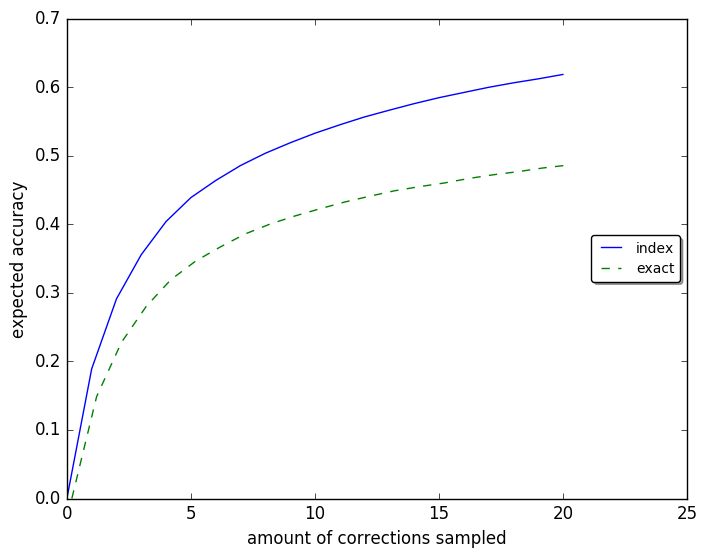
\includegraphics[width=\textwidth]{noSig_repeat_1000_accuracy}
		\caption{Accuracy and Exact Index Match.
			%Each data point is paired with a confidence interval ($p=.95$).     
		} \label{fig:accuracy_vals}
	\end{subfigure}
	\hfil
	\begin{subfigure}[]{0.65\columnwidth}
		\centering
		\includegraphics[width=\textwidth]{$F_{0.5}$_GLEU_Ms_significance}
		\caption{$F_{0.5}$ and GLEU\label{fig:F_Ms}}
	\end{subfigure}
	\hfil
	\begin{subfigure}[]{0.65\columnwidth}
		\centering
		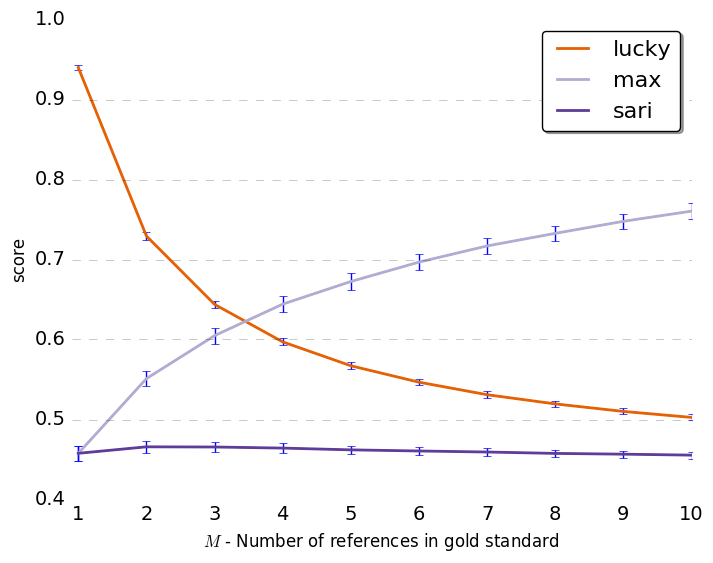
\includegraphics[width=\textwidth]{lucky,max,sari_Ms_significance}
		\caption{
			lucky\textbackslash perfect SARI and MAX-SARI\label{fig:SARI_Ms}}
	\end{subfigure}
	%\vspace{-0.2cm}
	\caption{Analysis (left) and empirical experiments (mid, right) to measure values for a perfect system (y-axis)
		as a function of the number of references $M$ (x-axis). For bootstrapping experiments points are paired with a confidence interval ($p=.95$).}
	%\vspace{-0.5cm}
\end{figure*}

Figure \ref{fig:accuracy_vals} presents the expected accuracy of a perfect
system (i.e., 1-$\hat{b}_M$) for different  $M$s. 
Results show that even for $M$ values which are much larger than the standard (e.g., $M=20$),
expected accuracy is only around 0.5. As $M$ increases, the contribution of each additional correction 
diminishes sharply (the slope is 0.004 for $M=20$).

We also experiment with a more relaxed measure, {\it Exact Index Match}, which is only sensitive to the identity of the changed words and not to what they were changed to. 
Formally, two corrections $c$ and $c'$ over a source sentence $x$ match if for their word alignments with the source (computed as above) $a:\{1,...,\left|x\right|\} \rightarrow \{1,...,\left|c\right|,Null\}$
and $a':\{1,...,\left|x\right|\} \rightarrow \{1,...,\left|c'\right|,Null\}$, it holds that $c_{a\left(i\right)} \neq x_{i} \Leftrightarrow c'_{a'\left(i\right)} \neq x_{i}$, where $c_{Null}=c'_{Null}$.
Results, while somewhat higher, are still only 0.54 with $M=10$. (Figure \ref{fig:accuracy_vals})
%As Exact Index Match can be interpreted as an accuracy measure for GED, this indicates that GED evaluation suffers from similar difficulties.

	%\vspace{-0.2cm}
\paragraph{$F$-Score.}
While accuracy is commonly used as a loss function for training GEC systems,
$F_\alpha$-score is standard for evaluating system performance.
The score is computed in terms of {\it edit} overlap between edits that constitute a correction and ones that constitute a reference, where edits are sub-string replacements to the source.
%The HOO shared task used an earlier version of $F$-score, which required that the proposed corrections include edits explicitly.
%Later on, relieving correctors from the need to produce edits, 
We use the standard $M^2$ scorer \cite{dahlmeier2012better}, which defines edits optimistically, maximizing over all possible annotations that generate the correction 
from the source. Since our crowdsourced corrections are not annotated for edits, we produce edits to the reference heuristically.
%$M^2$  is the standard $F$-score scorer for GEC.

The complexity of the measure prohibits an analytic approach \cite{yeh2000more}.
We instead use bootstrapping to estimate the bias incurred by not being able to exhaustively enumerate the set of valid corrections.
As with accuracy, in order to avoid confounding our results with system-specific biases,
we assume the evaluated system is perfect and sample its corrections from the human distribution of corrections $\mathcal{D}_x$.

Concretely, given a value for $M$ and for $N$, we uniformly sample from our experimental corpus source sentences $x_1,...,x_N$, and $M$ corrections for each $Y_1,...,Y_N$ (with replacement).
Setting a realistic value for $N$ in our experiments is important for obtaining comparable results to those obtained on the NUCLE corpus (see \S\ref{sec:real_world}),
as the expected value of $F$-score depends on $N$ and the number of sentences that do not need correction ($N_{cor}$).
Following the statistics of NUCLE's test set, we set $N=1312$ and $N_{cor}=136$.
%The latter reduces the overall bias by their frequency in the corpus.

Bootstrapping is carried out by the accelerated bootstrap procedure \cite{efron1987better}, with 1000 iterations.
We also report confidence intervals ($p=.95$), computed using the same procedure.%\footnote{We use the Python scikits.bootstrap implementation.}
%
%For each sentence which had at least one error according to the NUCLE gold standard
%we sample $M$ sentences uniformly from the
%gathered empirical data to replace it. We leave sentences that do not need
%corrections untouched. This results in reference texts accounting for the
%variability in different choices of corrections while approximating the reduction of variability
%of a big $N$ by consisting of $N$ sentences overall.

Results (Figure \ref{fig:F_Ms}) again show the insufficiency of commonly-used
$M$ values for reliably estimating system performance.
For instance, the $F_{0.5}$-score for our perfect system is only 0.42 with $M=2$.
The saturation effect, observed for accuracy, is even more pronounced in this setting.

%\vspace{-.2cm}
\paragraph{GLEU.} We repeat the procedure using the mean GLEU sentence score (Figure \ref{fig:F_Ms}), 
which was shown to better correlate with human judgments than $M^2$ \cite{napoles-sakaguchi-tetreault:2016:EMNLP2016}.
Results are about $2\%$ higher than $M^2$'s with a similar saturation effect.
\citet{sakaguchi2016reassessing} observed a similar effect when evaluating system outputs against fluency-oriented references,
which led them to assume that saturation is due to covering most of the probability mass,
which we now show is not the case.\footnote{
We do not experiment with I-measure \cite{felice2015towards}, 
as its run-time is prohibitively high for experimenting with bootstrapping
that requires many applications of the measure, and as empirical validation 
studies showed that it has a low correlation with human judgments \cite{sakaguchi2016reassessing, choshen2018maege}.}


%%%%%%%%%%%%%%%%%%%%%%%%%%%%%%%%%%%%%%%%%%%%%%%%%%%%%%%%%%%%%%%%%%%%%%%%%%%%%
	%\vspace{-0.1cm}
\subsection{Human and System Performance}\label{sec:real_world}
	%\vspace{-0.1cm}

The bootstrapping method for computing the significance of the $F$-score (\S\ref{subsec:Assessment-values}) 
can also be used for assessing the significance of the differences in system performance reported in the literature.
We compute confidence intervals of different systems on the NUCLE
test data ($M=2$).
 %report results %with the bootstrapping protocol 

\begin{figure}
  \includegraphics[width=0.9\columnwidth]{$F_{0.5}$_significance}
  \caption{$F_{0.5}$ values with $M=2$ for different systems, including confidence interval ($p=.95$).
    The left-most column (``source'') presents the $F$-score of a system that doesn't make any
    changes to the source sentences. In red is human performance.
    See \S \ref{par:experimental_setup} for a legend of the systems.\label{fig:F_correctors}}
%\vspace{-0.5cm}
\end{figure}

Results (Figure \ref{fig:F_correctors}) present mixed trends: some
differences between previously reported $F$-scores are indeed significant and some are not.
For example, the best performing system is significantly better than all but the second one.

Considering the $F$-score of the best-performing systems, and comparing 
them to the $F$-score of a perfect system with $M=2$ (in accordance with systems' reported results),
we find that their scores are comparable, where the systems RoRo and JMGR surpass a perfect system's $F$-score.
Similar experiments with GLEU show that the two systems obtain comparable or superior performance to humans
on this measure as well.

%
%Nevertheless, it seems that $M=2$ value taken in NUCLE is sufficiently high
%to generally obtain statistically significant ranking of the different correctors.

	%\vspace{-0.1cm}
\subsection{Discussion}\label{subsec:mult_discussion}
	%\vspace{-0.1cm}
	
% -- we saw that we have dramatic under-estimation
% -- but is this a problem? for instance, in the last section we saw we can get statistical significance between systems by increasing
%    N even with a low $M$
% -- balancing $N$ and $M$ is important;
%      other people have looked at similar things (not to re-label or not to re-label). we stress that
%      while for statistical significance increasing $N$ is sufficient, this would not solve this problem:
% -- low coverage entails other problems: it incentivizes systems not to correct, even if they can perfectly predict valid corrections.
% -- mathematical argument
% -- indeed, we see RoRo > Perfect and other systems are close to Perfect. it could be that they are better tailored to
%    those corrections produced by the NUCLE annotators. however in section 2 we saw that they are not.
%    we hypothesize that this is the reason.
%
%We have shown the number of corrections needed for reliable RBMs is exceedingly high.
%An average sentence has hundreds or more valid low-probability corrections, whose total probability mass is substantial. RBMs such as accuracy and $F$-score thus increase slowly with $M$ over 10.

%All these findings suggest that it is too costly to increase $M$ in development data to the extent asymmetric evaluation will seize to be influential. The exact index match analysis also suggests $M=1,2$ coverage is also low for detection. %When detection is separate from correction this might result in over-conservatism. 
%
%about a quarter of the probability mass of valid corrections (\S \ref{subsec:Assessment-values}).
%
%The factors controlling significance are two. Variation across sentences themselves (different $D_x$)
%which is reduced with $N$ and the variation across choices of corrections which might be reduced with
%either $M$ or $N$. One can rightly deduce that large $N$ is sufficient for variation, but it will not
%solve the other problems: under-estimation of true performance,
%over-conservatism, possible issues when training systems, and might be more costly than annotating
%a larger $M$ without acquiring more sentences and also annotating them.
%Choosing how to balance is dependent on the goals of the one collecting data, and affects over
%the mean value as well, as discussed in \ref{subsec:Assessment-values}. Thus, we bring supporting data and
%leave the decision to the reader. 

% Two recent RBMS have been proposed. One is {\sc I-measure} \cite{felice2015towards}, which introduces novel features to GEC evaluation, such as distinguishing different quality levels of ungrammatical corrections (e.g., some improve the quality of the source, while others degrade it), and restricting edits to only consist of single words, rather than phrases. The other is GLEU \cite{napoles2015ground}, an adaptation of BLEU that was shown to correlate well with human rankings. 

%Hence, there is no balance between overlooking mistakes and punishing valid corrections.

%The $F$-score coverage experiment echo the results of \newcite{bryant2015far},
%who also compared the $F$-score of a human correction against an increasing number of references.
%However, their suggestion to normalize the score
%with the score of a human corrector cannot address the gaps discussed here,
%as it has no effect on the training and tuning phases.
%Moreover, such normalization may be disadvantageous given that some systems already
%surpass human performance,
%indicating that addressing the biases incurred by limited coverage is not only a matter of scale.


%Also, changing from grammatical corrections to fluency ones results in more possible corrections, and consequently a larger bias.
%\lc{we repeat that to emphasize, right? I removed it from the introduction, it seems like too much focus on something that seems like a smaller criticism than before (they did not do it for simplification, for other measures, for dev and train, failed to miss what we see etc.) should it still occur twice in the paper? if not perhaps remove is from the f score paragraph and combine here.}
%Finally, note that addressing under-estimation by comparing to
%a human expected score (perfect corrector) with the same $M$ \cite{bryant2015far},
%does not address over-conservatism, it only scales the original measure. Moreover, as seen above, a human correction's score
%is not necessarily an upper bound, as an over-conservative corrector may surpass a perfect corrector in score.

%	Our findings echo the results of \newcite{bryant2015far}, who study the effect of $M$ on $F$-score, but the additional results in this paper suggests that their solution is still lacking. 
	%who study the effect of $M$ on $F$-score, the most commonly used measure for GEC.
%Our findings echo the results of \newcite{bryant2015far}, who study the effect of $M$ on $F$-score, the most commonly used measure for GEC. Their work focused on obtaining a more reliable estimate of correctors' performance and proposed to do so by normalizing corrector's estimated performance with the performance of a human corrector.

In this section we have established that (1) as systems can surpass human performance on RBMs, re-scaling cannot
be used to overcome the LCB, and that (2) as the distribution of valid corrections is long-tailed, 
the number of references needed for reliable RBMs is exceedingly high.
Indeed, an average sentence has hundreds or more valid low-probability corrections, whose 
total probability mass is substantial. %RBMs such as accuracy and $F$-score thus increase slowly with $M$ over 5. 
Our analysis with Exact Index Match suggests that similar effects are applicable to Grammatical Error Detection as well.
The proposal of \newcite{sakaguchi2016reassessing}, to emphasize fluency over grammaticality in reference corrections, 
only compounds this problem, as it results in a larger number of valid corrections.

%These results suggest that alternative methods that do not apply string similarity between the source and the references 
%may be more effective in addressing LCB. 
%In recent ongoing work we suggest\lc{[perhaps needs to be anonymized if the Usim would be published by then]} USim \citet{us} a reference-less evaluation measure which by definition does not suffer from this biases.


%\vspace{-.1cm}
\section{Implications of the LCB}\label{sec:formal_conservatism}
%\vspace{-.1cm}

We discuss the adverse effects of LCB not only on the reliability of RBMs, but on the development
of GEC systems.
We argue that evaluation with inadequate reference coverage incentivizes systems to under-correct,
and to mostly target errors that have few valid corrections (closed-class).
We first show that low coverage can lead to under-correction (\S\ref{subsec:motivating_analysis}),
then show that modern systems make far fewer corrections to the source, compared to humans (\S\ref{subsec:under-correction}).
\S\ref{subsec:reranking} shows that increasing the number of references can alleviate this effect.
\S\ref{subsec:by_types} shows that open-class errors are more likely to be under-corrected than closed-class ones.

%\vspace{-.1cm}
\subsection{Motivating Analysis}\label{subsec:motivating_analysis}
%\vspace{-.1cm}

For simplicity, we abstract away from the details of the learning model and assume 
that systems attempt to maximize an objective function, 
over some training or development data. 
We assume maximization is achieved by iterating over the samples, as with the Perceptron or SGD.

Assume the system is faced with a phrase it predicts to be ungrammatical. 
Assume $p_{detect}$ is the probability this prediction is correct, and
$p_{correct}$ is the probability it is able to predict
a valid correction for this phrase (including correctly identifying it as erroneous).
Finally, assume evaluation is
against $M$ references with coverage $p_{coverage}$
(the probability that
a valid correction will be found among $M$ randomly sampled references).

We will now assume that the system may either choose to correct with the correction it finds 
the most likely or not at all. If it chooses not to correct, its probability of being rewarded 
(i.e., its output is in the reference set) is $(1-p_{detect})$. Otherwise, its probability
of being rewarded is $p_{correct} \cdot p_{coverage}$.
A system is disincentivized from altering the phrase in cases where:

%\vspace{.1cm}
\begin{small}
	\begin{myequation}
		\label{eq:reward}
		p_{correct} \cdot p_{coverage} < 1-p_{detect} 
	\end{myequation}
	%\vspace{-.1cm}
\end{small}


We expect Condition (\ref{eq:reward}) to frequently hold in cases that
require non-trivial changes, which are characterized both by low $p_{coverage}$ (as non-trivial
changes are often open-class), and by lower system performance.

Precision-oriented measures (e.g., $F_{0.5}$) penalize invalidly correcting more
harshly than not correcting an ungrammatical sentence.
In these cases, Condition (\ref{eq:reward}) should be written as

\begin{small}
	%\vspace{-.1cm}
	\begin{myequation*}
		p_{correct} \cdot p_{coverage} - \left(1-p_{correct} \cdot p_{coverage}\right) \alpha < 1-p_{detect} 
	\end{myequation*}
	%\vspace{-.1cm}
\end{small}

\noindent
where $\alpha$ is the ratio between the penalty for introducing a wrong correction and the reward for a valid correction. The condition is even more likely to hold with such measures.


%%%%%%%%%%%%%%%%%%%%%%%%%%%%%%%%%%%%%%%%%%%%%%%%%%%%%%%%%%%%%%%%%%%%%%%%%%%%%%%%%%%%%%%%%%%%%%%%%%%%%%%%%
%\vspace{-.1cm}
\subsection{Under-correction in GEC Systems}\label{subsec:under-correction}
%\vspace{-.1cm}
\begin{table}
	%\vspace{-0.5cm}
	\centering
	\small
	\singlespacing
	\begin{tabular}{l|p{4cm}}
		Corrector & Sentence \\
		\hline
		Source & This is especially to people who are overseas. \\
		\hline 
		CHAR, UMC, JMGR & This is especially \textbf{for} people who are overseas. \\ 
		IPN & This is especially to \textbf{peoples} who are overseas. \\ 
		CUUI &  This is especially to \textbf{the} people who are overseas. \\ 
		\hline
		NUCLE$_A$ & This is especially \textbf{true for} people who are overseas.\\
		NUCLE$_B$ & This is especially \textbf{relevant} to people who are overseas.
	\end{tabular}
	\caption{\label{tab:nucle_example} Example for a sentence and proposed corrections by different systems (top part) and by the two NUCLE annotators (bottom part). Systems not mentioned in the table retain the source. No system produces a new word as needed. The two references differ in their corrections.} 
	%\vspace{-0.5cm}
\end{table} 

In this section we compare the prevalence of changes made to the source by the systems,
to their prevalence in the NUCLE references (one annotator was arbitrarily 
selected for the figures). 
%\newcite{bryant2015far} noticed that the NUCLE references are more conservative than 
%the ones they collected, which implies that our results may even underestimate the level 
%of conservatism relative to other references.
To strengthen our claim, we exclude all non-alphanumeric characters, 
both within tokens or as separate tokens. See Table \ref{tab:nucle_example} 
for an example.

We consider three types of divergences between the source and the reference.
First, we measure the extent to which \emph{words} were changed: altered, deleted or added.
To do so, we compute word alignment between the source and the reference, casting it
as a weighted bipartite matching problem. Edge weights are assigned to be the token edit distances.
(Aligning words in GEC is much simpler than in MT,
as most of the words are unchanged, deleted fully, added, or changed slightly.)
Following word alignment, we define {\sc WordChange}
as the number of aligned words and unaligned words changed.
Second, we quantify word \emph{order} differences using
Spearman's $\rho$ between the order of the words in the source sentence
and the order of their corresponding-aligned words in the correction.
$\rho=0$ where the word order is uncorrelated, and $\rho=1$ where the orders exactly match. We report the average $\rho$ over all source sentence pairs. 
Third, we report how many source sentences were split and how many concatenated by the reference and by the systems.

\begin{figure*}
	%\vspace{-0.8cm}
	\centering
	\begin{subfigure}[]{0.6\columnwidth}
		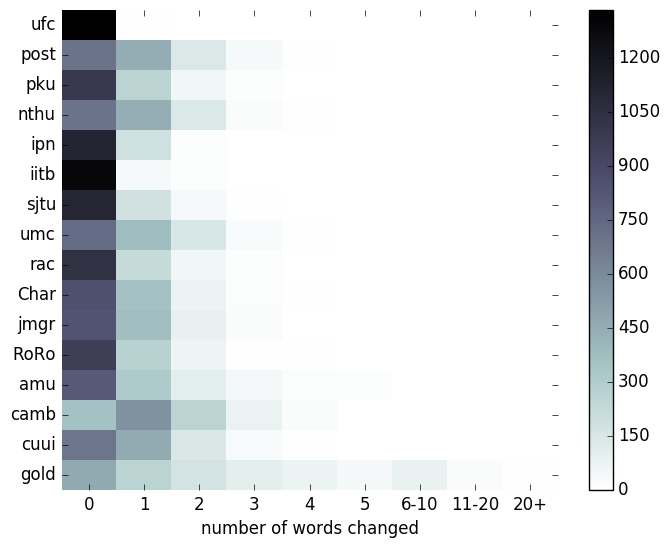
\includegraphics[width = \textwidth]{words_differences_heat}
	\end{subfigure}
	\hfill
	\begin{subfigure}[]{0.6\columnwidth}
		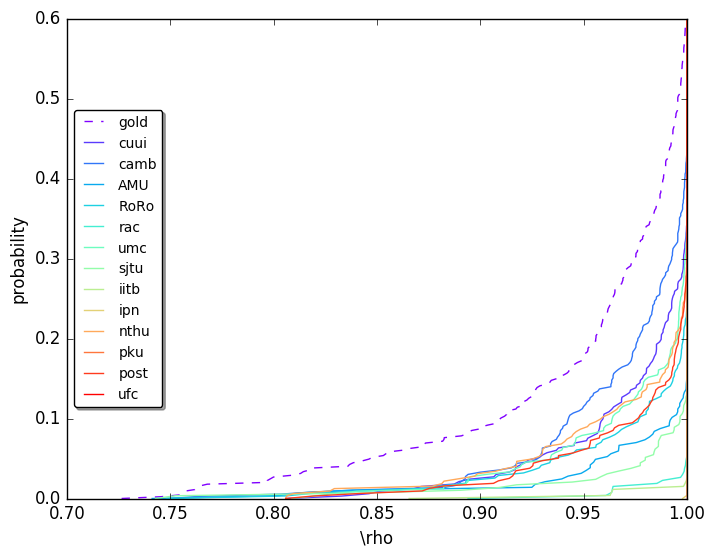
\includegraphics[width = \columnwidth]{spearman_ecdf}
	\end{subfigure}
	\hfill
	\begin{subfigure}[]{0.6\columnwidth}
		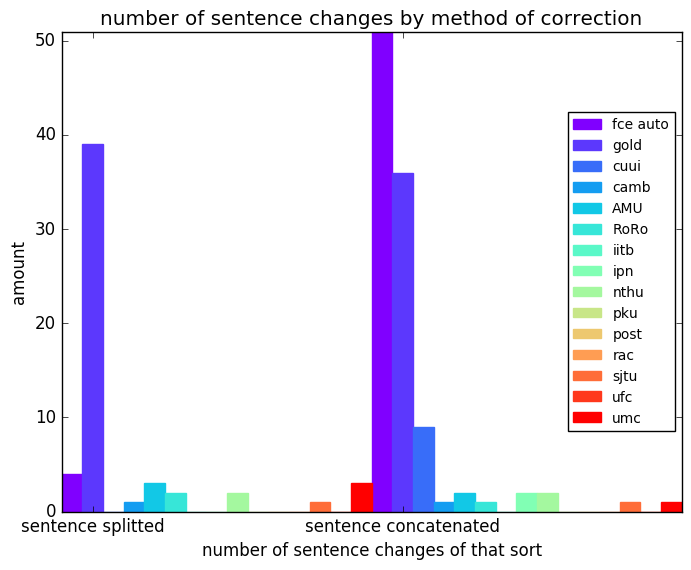
\includegraphics[width = \textwidth]{aligned}
	\end{subfigure}
	\caption{\label{fig:over-conservatism}
		The prevalence of changes in system outputs and in the NUCLE reference.
		The left figure presents the number of sentences (heat) for each amount of word changes
		(x-axis; measured by {\sc WordChange}) done by the outputs and the reference (y-axis).
		The middle figure presents the percentage of sentence pairs (y-axis) where the
		Spearman $\rho$ values do not exceed a certain threshold (x-axis).
		The right figure presents the counts of source sentences (y-axis) concatenated (right bars) or split (left bars) by the references (striped column) and the outputs (coloured columns).
		See Appendix \ref{ap:abbr} for a legend of the systems.
		Under all measures, the gold standard references make substantially more changes to the source sentences than any of the systems, in some cases an order of magnitude more.
	}
	%\vspace{-0.35cm}
\end{figure*}

%\vspace{-.2cm}
\paragraph{Results.} \hspace{-.5cm}
Results (Figure \ref{fig:over-conservatism}) show that humans make considerably more changes than systems according to all measures of under-correction, 
both in terms of the number of sentences modified and the number of modifications within them. Differences are often an order of magnitude large.
For example, 36 reference sentences include 6 word changes, where the maximal number of sentences with 6 word changes by any system is 5.
We find similar trends on the references of the TreeBank of Learner English \cite{yannakoudakis2011new}.

%%%%%%%%%%%%%%%%%%%%%%%%%%%%%%%%%%%%%%%%%%%%%%%%%%%%%%%%%%%%%%%%%%%%%%%%%%%%%%%%%%%%
%\vspace{-.2cm}
\subsection{Higher $M$ Alleviates Under-correction}\label{subsec:reranking}

This section reports an experiment for determining whether increasing
the number of references in training indeed reduces under-correction. There is no 
corpus available with multiple references which is large enough for re-training a system. 
Instead, we simulate such a setting with an oracle reranking approach, and test whether the 
availability of increasingly more training references reduces a system's under-correction.

Concretely, given a set of sentences, each paired with $M$ references, a measure and a 
system's $k$-best list, we define an oracle re-ranker that selects for each sentence the highest scoring correction.
As a test case, we use the RoRo system with $k=100$, and apply it to the 
largest available language learner corpus which is paired with a substantial amount of GEC references,
namely the NUCLE test corpus. We use the standard $F$-score as the evaluation measure,
examining the under-correction of the oracle re-ranker for different $M$ values, averaging over the 1312 samples of 
$M$ references from the available set of ten references provided by \citet{bryant2015far}.

\textcolor{red}{As the argument is not trivial, we turn to explain }why decreased under-correction with an increase in $M$ indicates
that tuning against a small set of references (low coverage) yields under-correction. 
Assume an input sentence with some sub-string $e$. 
There are three cases: (1) $e$ is an error, (2) $e$ is valid but there are valid references that alter it, (3) $e$ is uniquely valid. In case (3) oracle re-ranking has no effect and can be ignored.
%In cases (1) and (2), denote the set of valid corrections of $e$ as $E$.
The corrections in the $k$-best list can then be partitioned to those that keep $e$ as it is; those that invalidly alter $e$; and those that validly alter $e$. 


\begin{table}[t]
	%\vspace{-0.5cm}
	\centering
	\small
	\singlespacing
	\begin{tabular}{c|c|cc}
		& $L_{val}$ empty & \multicolumn{2}{c}{$L_{val}$ not empty} \\
		&            & $e$ valid & $e$ error \\ \hline
		\multicolumn{1}{c|}{Small $M$} & 0 & $P_Y(\overline{e}, L_{val})$ & $P_Y\left(L_{val}\right)$    \\
		\multicolumn{1}{c|}{Large $M$} & 0 & 0              & 1                  \\ \hline
		\multicolumn{1}{c|}{Outcome}            & same  & $\downarrow$ changes        & $\uparrow$ changes
	\end{tabular}
	\caption{\label{ta:oracle_expected_results}
		The expected effect of oracle re-ranking on under-correction.
		Values represent the probability of altering a sub-string of the input $e$, \textcolor{red}{i.e., the probability that another sub-string in the $k$-best list scores higher than $e$} . $L_{val}$ is the valid alterations in the $k$-best list. $P_Y\left(L_{val}\right)$ is the probability that a valid correction from the list is also in the reference set $Y$,
		$P_Y(\overline{e}, L_{val})$ is the probability that, in addition, the reference that keeps $e$ is not in $Y$.
		% in the reference set ($Y$) and references from $L_{val}$ (that alter $e$) are selected in the reference set.. 
		%Cases include the case where the $k$-best list contains/not contains valid corrections of $e$,
		%and the cases where keeping $e$ is valid/not valid.
		%\vspace{-0.2cm}
	}
	%Results under different assumptions concerning the ability of correctors to correct, the need for correcting most of the errors, 
	%and the probability for high coverage with small $M$. 
	%$%P$ is the probability to be in $Y$. 
	
	
\end{table}

Table \ref{ta:oracle_expected_results} presents the probability that $e$ will be altered in the different cases.
Analysis shows that under-correction is likely to decrease with $M$ only
in the case where $e$ is an error and the $k$-best list contains a valid correction of it.
Whenever the reference allows both keeping $e$ and altering $e$, the re-ranker selects keeping $e$. 

%the only case where oracle re-ranking is expected to increase the number of changes
%is where both $e$ is an error and the $k$-best list contains valid corrections of $e$ ($L_{val} \neq \emptyset$).

Indeed, our experimental results show that word changes increase with $M$ (Figure \ref{fig:reranking_word_change}),
indicating that low coverage may play a role in the observed tendency of GEC systems to under-correct.
%the observed under-correction pattern is related to the low coverage of the reference set available  for re-ranking. 
No significant difference is found for word order.

%
\begin{figure}
	%\vspace{-1em}
	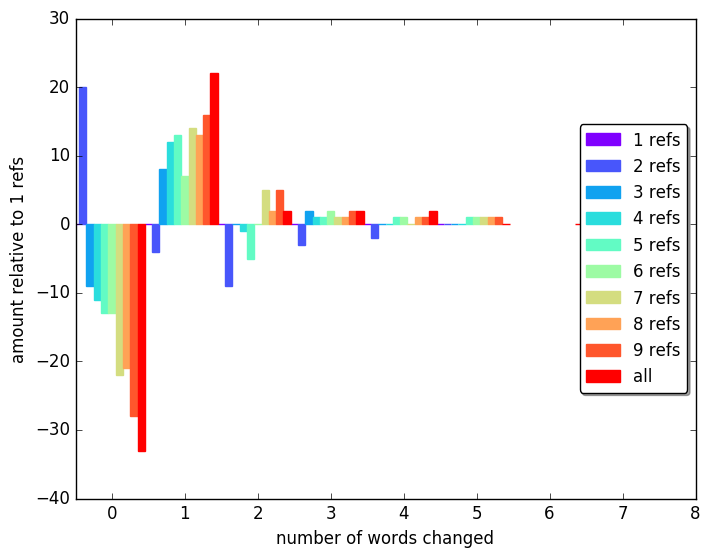
\includegraphics[width=0.9\columnwidth]{words_relative_differences_hist_reranking}
	\caption{The amount of sentences (y-axis) with a given number of words changed (x-axis) following oracle reranking with different $M$ values (column colors), 
	where the amount for $M=1$ is subtracted from them.
		All references are randomly sampled except the ``all'' column that contains all ten references.
		In conclusion, tuning against additional references indeed reduces under-correction.
		\label{fig:reranking_word_change}
	}
	%\vspace{-0.5cm}
\end{figure}

%The field of GEC was always thriving or conservatism in its corrections, with the prominent example of using
%$F_{0.5}$ emphasizing precision over recall(\cite{ng2014conll}). we wish to highlight the problem that
%arises from pursuing this conservatism as done today.
%Then, we wished to be conservative, and we achieved that, why shouldn't we rejoice just yet? Theoretically, we might be progressing towards not correcting at all, instead of progressing towards correcting more accurately. 
%
%Manual analysis showed excessive formal conservatism and under correction.
%Albeit important, manual analysis is not enough and we aimed for generating some quantitative measures. 
%
%We demonstrate that current correctors
%suffer from over-conservatism: they tend to make too few changes to the source, relative to human correctors.
%{ \color{red} This is likely an indication of some hidden, cross-systems, widely spread  bias.}


\subsection{Under-correction by Error Types}\label{subsec:by_types}

In this section we study the prevalence of under-correction according to edit types, finding that open-class types of errors
(such as replacing a word with another word) are more starkly under-corrected, than closed-class errors.
Evaluating with low coverage RBMs does not incentivize systems to address open-class errors (in fact, it disincentivizes them to). Therefore, even if LCB is not the cause for this trend, current evaluation procedures may perpetuate it.

We use the data of \citet{bryant-felice-briscoe:2017:Long}, which automatically assigned types to each correction in the output of all CoNLL 2014 
systems on the NUCLE test set.
As a measure of under-correction tendency, we take the ratio between the mean number of corrections produced by the systems and by the references as proposed by {\sc MAEGE} \cite{choshen2018maege}. 
We note that this analysis does not consider whether the predicted correction is valid or not, but only how many of the errors of each type the systems attempted to correct. 

We find that all edit types are under-predicted on average, but that the least under-predicted ones are mostly closed-class types. 
Concretely, the top quarter of error types consists of orthographical errors, 
plurality inflection of nouns, 
adjective inflections to superlative or comparative forms and determiner selection. The bottom quarter includes the categories 
verb selection, noun selection, particle/preposition selection, pronoun selection, and the type {\sc OTHER}, which is a residual category.
The only exception to this regularity is the closed-class punctuation selection type, which is found in the lower quarter. See Appendix \ref{ap:types}.

This trend cannot be explained by assuming that common error types are targeted more.
Indeed, error type frequency is slightly negatively correlated with the under-correction ratio ($\rho$=-0.29 p-value=0.16).
A more probable account of this effect is the disincentive of GEC systems to correct error types for which even valid
corrections are unlikely to be rewarded.

%%%%%%%%%%%%%%%%%%%%%%%%%%%%%%%%%%%%%%%%%%%%%%%%%%%%%%%%%%%%%%%%%%%%%%%%%%%%%%%%%%%%%
%\vspace{-.1cm}
\section{Similar Effects on Simplification}\label{sec:simplification}
%\vspace{-.1cm}

We now turn to replicating our experiments on Text Simplification (TS). 
From a formal point of view, evaluation of the tasks is similar:
the output is obtained by making zero or more edits to the source. RBMs are the standard for TS evaluation,
much like they are in GEC.

Our experiments on TS demonstrate that similar trends recur in this setting as well. 
The tendency of TS systems to under-predict changes to the source 
has already been observed by previous work \cite{alvamanchego-EtAl:2017:I17-1}, 
showing that TS systems under-predict word additions, deletions,
substitutions, and sequence shifts \cite{zhang-lapata:2017:EMNLP2017},
and have low edit distance from the source \cite{narayan-gardent:2016:INLG}.
Our experiments show that LCB may account for this under-prediction. Concretely, we show that
(1) the distribution of valid references for a given sentence is long-tailed; 
(2) common evaluation measures suffer from LCB, taking SARI \cite{Xu-EtAl:2016:TACL} 
    as an example RBM (similar trends are obtained with Accuracy); 
(3) under-prediction is alleviated with $M$ in oracle re-ranking experiments.

We crowd-sourced 2500 reference simplifications for 47 sentences, using the corpus and the annotation protocol of 
\newcite{Xu-EtAl:2016:TACL}, and applying {\sc UnseenEst} to estimate $\mathcal{D}_x$ (Appendix  \ref{ap:crowd}).
Table \ref{tab:simplifications_dist} shows that the expected number of references is even greater in this setting. 

Assessing the effect of $M$ on SARI, we find that SARI diverges from Accuracy and $F$-score
in that its multi-reference version is not a maximum over the single-reference scores, but some combination of them.
This can potentially increase coverage, but it also leads to an unintuitive situation: an output 
identical to a reference does not receive a perfect score, but rather the score depends on how similar the output is to the other
references. A more in-depth analysis of SARI's handling of multiple references is found in Appendix \ref{ap:sari-assum}.
In order to neutralize this effect of SARI, we also report results with MAX-SARI, which coincides with SARI on $M=1$, 
and is defined as the maximum single-reference SARI score for $M>1$.

\com{
\begin{figure}
	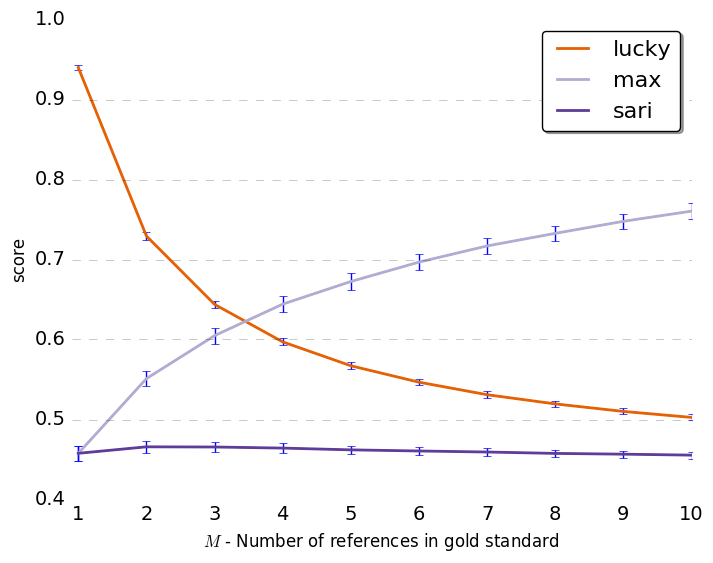
\includegraphics[width=0.9\columnwidth]{lucky,max,sari_Ms_significance}
	\caption{
		SARI and MAX-SARI values for a perfect system and SARI values for a ``lucky perfect'' system (y-axis) as a function of the number of references $M$ (x-axis).
		Each data point is paired with a confidence interval ($p=.95$).\label{fig:SARI_Ms}}
	%\vspace{-0.5cm}
\end{figure}
}

Figure \ref{fig:SARI_Ms} presents the coverage of SARI and MAX-SARI of a perfect TS system that selects a random correction
from the estimated distribution of corrections using the same bootstrapping protocol as in \S\ref{subsec:corrections_distribution}.
We also include the SARI score of a ``lucky perfect'' system, that randomly selects one of 
the given references (the MAX-SARI score for such a system is 1). 
Results show that SARI has a coverage of about $0.45$, and that this score is largely independent of $M$.
The score of predicting one of the available references drops with the number of references, indicating that SARI scores may not be comparable
across different $M$ values. 

We therefore restrict oracle re-ranking experiments to MAX-SARI, conducting re-ranking experiments on $k$-best
lists in two settings: Moses \cite{koehn2007koehn} 
with $k=100$, and a neural model \cite{nisioi2017exploring} with $k=12$. 
Our results indeed show that under-prediction is alleviated with $M$ in both settings. 
For example, the least under-predicting model (the neural one) did not change 50 sentences with $M=1$, but only 29 weren't changed 
with $M=8$. See Appendix \ref{ap:simp-rerank}.

%The results suggest that similar trends may hold for other monolingual translation tasks, at least to the extent that their RBMs take the source into account.
%, and compares the changes made to it in the references and the system output. This includes most measures for monolingual translation, excluding multilingual originated ones.

%The relation between coverage to conservatism in TS is further supported by 
%the fact that reduction in simplification conservatism came together with the use of the new corpus introducing references for tuning and a %more prominent change came with a semantic approach that can abstract over the references \cite{zhang-lapata:2017:EMNLP2017}.
%In our opinion, the above results attest to the need in considering coverage of evaluation procedures.

%We also tested oracle reranking using SARI. Two $k$-best list were used, simple moses based system ($k=100$) and a neural based one ($k=12$), while the first shows an inverse tendency, the second becomes less conservative. For example, for any number of changes $X$, the Moses system with $M=1$ has more sentences with at least $X$ corrections compared to reranking with $M=1$. We attribute this to lack valid corrections combined with SARI's behaviour. Conversely, the neural system with $M=1$ chose not to correct 50 sentences while the one with $M=8$ 30, exactly like the gold standard. 

\begin{table}[t]
	%\vspace{-0.5cm}
	\centering
	\small
	\singlespacing
	\begin{tabular}{c|c|c|c|c|}
		%\cline{2-5} 
		& \multicolumn{4}{c|}{Frequency Threshold ($\gamma$)}\\ 
		%\cline{2-5} 
		& \multicolumn{1}{c}{0} & \multicolumn{1}{c}{0.001} & \multicolumn{1}{c}{0.01} & \multicolumn{1}{c|}{0.1}
		\\
		\hline
		Variants & 2636.29 & 111.19 & 4.68 & 0.13
		\\
		Mass & 1 & 0.42 & 0.14 & 0.02\\
		\hline
	\end{tabular}
	\caption{\label{tab:simplifications_dist}
		Estimating the distribution of simplifications $\mathcal{D}_x$.
		The table presents the mean number of simplifications per sentence with probability more than
		$\gamma$ (top row), as well as their total probability mass (bottom row).
	}
	%\vspace{-0.5cm}
\end{table}
\lc{originally we wanted to move some TS text from the supplementary to here, given the reviews (stating we are too dense) should we reconsider? Do we have a way of a last effort for making the article easier to comprehend?}
%%%%%%%%%%%%%%%%%%%%%%%%%%%%%%%%%%%%%%%%%%%%%%%%%%%%%%%%%%%%%%%%%%%%%%%%%%%%%%%%%%%%%%
	%\vspace{-0.1cm}
\section{Conclusion}\label{sec:conclusion}
	%\vspace{-0.1cm}

%This paper addresses the shortcomings of existing RBMs in GEC.
%We present evidence that state of the art systems suffer from over-conservatism and
%argue that this over-conservatism results from developing, training and tuning them against measures that
%not only more harshly penalize undue corrections over under-correction,
%but also often penalize perfectly valid outputs.
%In fact, systems are often more likely to be penalized for a valid change than 
%to receive credit for it, due to the small number of references taken into account.
%Moreover, we show that a coverage-conservatism relation is not confined to
%GEC, and may be applicable to monolingual translation in general.

%Estimating the distribution of valid corrections for a sentence, we find
%that increasing $M$ is beneficial up to a point, after which
%coverage improves only marginally with each additional reference.

We argue that low-coverage reference sets has adverse effects on the reliability
of reference-based evaluation, \textcolor{red}{with GEC and TS as a test case,} and consequently on the incentives offered to systems.
We further argue that these effects cannot be overcome by re-scaling or increasing the number of references in a feasible way. 
The paper makes two methodological contributions to the \textcolor{red}{monolingual translation} evaluation literature:
(1) a methodology for evaluating evaluation measures by the scores they assign a perfect system, using a bootstrapping procedure;
(2) a methodology for assessing the distribution of valid monolingual translations.
Our findings demonstrate how these tools can help characterize the biases of existing systems and evaluation measures.
\textcolor{red}{We believe our findings and methodologies are useful for many similar tasks such as \lc{what is the task name, style generation? conversion? did not find it as a name of a task} style and automatic post-editing of raw outputs by MT.}

We note that the LCB further jeopardizes the reliability of common validation experiments for RBMs,
that assess the correlation between human and measure rankings of system outputs \cite{grundkiewicz2015human}.
Indeed, if outputs all similarly under-correct, correlation studies will not be affected by whether an RBM is sensitive to under-correction.
Therefore, the tendency of RBMs to reward under-correction, that we report here, 
cannot be detected by such correlation experiments \textcolor{red}{(For a complementary view on the subject see \cite{choshen2018maege})}.

Our results underscore the importance of developing alternative evaluation measures that transcend $n$-gram overlap, 
and use deeper analysis tools, e.g., by comparing
the semantics of the reference and the source to the output \cite[cf.][]{lo2011meant}.
\newcite{napoles-sakaguchi-tetreault:2016:EMNLP2016}
have made progress towards this goal in proposing a reference-less grammaticality measure,
using Grammatical Error Detection tools, \newcite{asano2017reference} added a fluency measure to the grammaticality.
In a recent project \cite{choshen2018usim}, we proposed a complementary measure that 
measures the semantic faithfulness of the output to the source, in order to form a combined semantic measure that bypasses the pitfalls of low coverage.


%A concluding note: RBMs are often validated by their correlation with human judgments, while the measures' absolute score is deemed as less important. 
%We show that the caveats of using low reference coverage are not a matter of scale, but rather that
%low coverage leads to systematic biases, which have a negative effect on system performance.
%Our oracle re-ranking experiments suggest that incorporating additional references into the training and tuning protocol may alleviate this problem. 
%As no corpus with multiple references is large enough to train GEC systems,
%we are currently pursuing the semi-automatic generation of such corpora, in order to develop methods
%for training GEC systems with multiple references, thereby overcoming over-conservatism.


%
% In many of the uses for correction, the user does know his grammar is not perfect and
% would accept a change in grammar when needed.
% Because of this approval we also hypothesis, and it may call for a user study to prove or disprove this hypothesis, that users might accept a correct text unit of theirs being corrected to another correct text unit with the same meaning.
% This would be an example of being faithful but not conservative.
%Maybe even more importantly, we aim to have as many correct sentences as possible, but as neither the grammar is fully correct in the first place, nor is the user's understanding of it, failing to correct grammar is acceptable. Changing meaning will be totally unacceptable, and also surely detectable by the user. In other words, the users do expect the corrector to be active and not too conservative, but only as long as it is faithful. 
%
%Moreover, as correctors are based on statistics, they might even
%just correct to a more common way of saying the same thing. Such unnecessary
%correction is not conservative, and at GEC maybe be unwanted, but not strictly unwanted as overall
%it is still faithful. Additionally, some may even
%consider such correction a needed one because it has a better grammar considering
%Fuzzy Grammar\cite{lakoff1973fuzzy,madnani2011they} or a more fluent
%way to say the exact same thing. The latter was recently suggested as a necessary
%shift in the goals of GEC\cite{sakaguchi2016reassessing}.
%Considering all this, we propose that next generation correctors and evaluation will be focused on faithfulness
%when possible rather than on conservatism. Of course that with the evaluation comes the development
%and it all suggests that it might be beneficial to incorporate faithfulness not only for assessment
%but also as a feature for correctors. 
%

%\lc{Suggest to delete this too:}
%Future work will assess the relative importance, ascribed by users of GEC systems,
%to different evaluation criteria of the output.
%Specifically, we will explore to what extent users are
%tolerant to changes in the sentence structure, i.e.,
%violation of conservatism, relative to their tolerance to changes in the sentence's meaning,
%i.e., violation of faithfulness.
%%A better understanding of how these interact
%may lead to improved semantic evaluation, that will alleviate the need
%for a high number of references.
\section*{Acknowledgments}

This work was supported by the Israel Science Foundation (grant No. 929/17),
and by the HUJI Cyber Security Research Center in conjunction with the Israel
National Cyber Bureau in the Prime Minister's Office.
We thank Nathan Schneider for helpful feedback and a different way of looking at our findings.

\bibliographystyle{acl_natbib}
\bibliography{propose}



\end{document}
